\textbf{مورد استفاده:}
پرداخت هزینه پروژه
\\
\textbf{شرح مختصر :UC}
در این قسمت کارفرما هزینه انجام پروژه توسط فریلنسر را پرداخت می‌کند.
\\
\textbf{پيش شرط:}
ورود به مدیریت مالی در داشبورد کارفرما.
\\
\textbf{سناريو اصلی:}
\begin{enumerate}
\item
شروع
\item
کارفرما بعد از انتخاب پروژه، دکمه پرداخت هزینه پروژه را انتخاب می‌کند و سیستم فرم پرداخت را به کارفرما نمایش می‌دهد.
\item
کارفرما فرم را تکمیل می‌کند و با دکمه ارسال، فرم تکمیل شده را به سیستم ارسال می‌کند.
\item
سیستم اطلاعات فرم را بررسی می‌کند و اطلاعات را به بانک عامل ارسال می‌کند.
\item
اطلاعات پرداخت دریافت می‌شود و در بانک اطلاعات ثبت می‌شود.
\item
پایان
\end{enumerate}

\noindent
\textbf{پس شرط:}
وجه بعد از انتخاب فریلنسر جهت ضمانت در سایت بلوکه می‌شود.
\\
\textbf{سناريوهای فرعی:}
\\
\textbf{سناريو فرعی 1:}
خطا در اطلاعات فرم پرداخت
\\
\textbf{شرح مختصر :UC}
این سناریو در مرحله 4 سناریو اصلی در صورت خطا در اطلاعات فرم اجرا می‌شود.
\begin{enumerate}
\item
شروع
\item
اطلاعات فرم بررسی می‌شود و خطاها مشخص می‌شوند.
\item
یک پیغام به کارفرما نمایش داده می‌شود و درخواست اصلاح اطلاعات فرم را دارد.
\item
از مرحله 3 سناریو اصلی ادامه پیدا می‌کند.
\item
پایان
\end{enumerate}

\noindent
\textbf{سناريو فرعی 2:}
خطا در پرداخت وجه
\\
\textbf{شرح مختصر :UC}
این سناریو در مرحله 5 سناریو اصلی در صورت خطا در پرداخت اجرا می‌شود.
\begin{enumerate}
\item
شروع
\item
اطلاعات خطا از طرف بانک عامل به سیستم ارسال می‌شود.
\item
یک پیغام به کارفرما نمایش داده می‌شود و ناموفق بودن پرداخت را اعلام می‌کند.
\item
از مرحله 2 سناریو اصلی ادامه پیدا می‌کند.
\item
پایان
\end{enumerate}

\noindent
\textbf{سناريو فرعی 3:}
با موفقیت پرداخت ‌شود
\\
\textbf{شرح مختصر :UC}
این سناریو در مرحله ۴ سناریو اصلی در صورت موفقیت آمیز بودن پرداخت اجرا می‌شود.
\begin{enumerate}
\item
شروع
\item
اطلاعات پرداخت از طرف بانک عامل به سیستم ارسال می‌شود.
\item
یک پیغام به کارفرما نمایش داده می‌شود که پرداخت با موفقیت انجام شده است.
\item
از مرحله 4 سناریو اصلی ادامه پیدا می‌کند.
\item
پایان
\end{enumerate}

\noindent
\textbf{پس شرط:}
ندارد.




\begin{figure}[H]
	\centering
	\includegraphics[width=.9\textwidth]{Diagram/2.Activity/کارفرما/مدیریت-مالی-پرداخت.png}
	\caption{دیاگرام فعالیت پرداخت هزینه}
	\label{fig:a:پرداخت-هزینه}
\end{figure}
\begin{figure}[H]
	\centering
	\includegraphics[width=.8\textwidth]{Diagram/3.StateMachine/کارفرما/مدیریت-مالی-پرداخت.png}
	\caption{دیاگرام حالت ماشین پرداخت هزینه}
	\label{fig:sm:پرداخت-هزینه}
\end{figure}
\begin{figure}[H]
	\centering
	\includegraphics[width=1\textwidth]{Diagram/4.Collaboration/1.Sequence/کارفرما/مدیریت-مالی-پرداخت.png}
	\caption{دیاگرام توالی پرداخت هزینه}
	\label{fig:s:پرداخت-هزینه}
\end{figure}
\begin{figure}[H]
	\centering
	\includegraphics[width=1\textwidth]{Diagram/4.Collaboration/2.Communication/کارفرما/مدیریت-مالی-پرداخت.png}
	\caption{دیاگرام همکار پرداخت هزینه}
	\label{fig:c:پرداخت-هزینه}
\end{figure}
